\documentclass[10pt]{article}
\usepackage[margin=0.62in]{geometry}
\usepackage{graphicx}
\usepackage{booktabs}
\usepackage{multicol}
\usepackage{hyperref}
\title{\vspace{-1.2cm}SmartFlow: Adaptive Traffic Signal Control with Reinforcement Learning}
\author{Group 19}
\date{}

\begin{document}
\maketitle
\vspace{-0.5cm}

\section*{1. Motivation and Part I Formulation}
Urban congestion is a sequential decision-making problem under stochastic arrivals. Fixed-cycle traffic lights cannot adapt to changing queues, while reinforcement learning (RL) can learn policies that trade immediate clearance against future congestion. The original presentation modeled a single intersection as a Markov Decision Process with state
\[
S=(Q_{NS},Q_{EW},Phase),
\]
where each queue is bucketed into Low $(0$--$3)$, Medium $(4$--$8)$, or High $(9+)$. The action set is \{Stay, Switch\}. The reward is
\[
R=-(Q_{NS}+Q_{EW})-C,
\]
where switching incurs a small penalty to discourage unsafe oscillation. The algorithms compared were Q-Learning, SARSA, Monte Carlo, static fixed-cycle timing, a greedy longest-queue heuristic, and a Value Iteration reference.

\section*{2. Preserved Part I Results}
The Part I values below are preserved exactly from the presentation's Experiment Results slide and regenerated from \texttt{presentation\_results.csv}.

\begin{center}
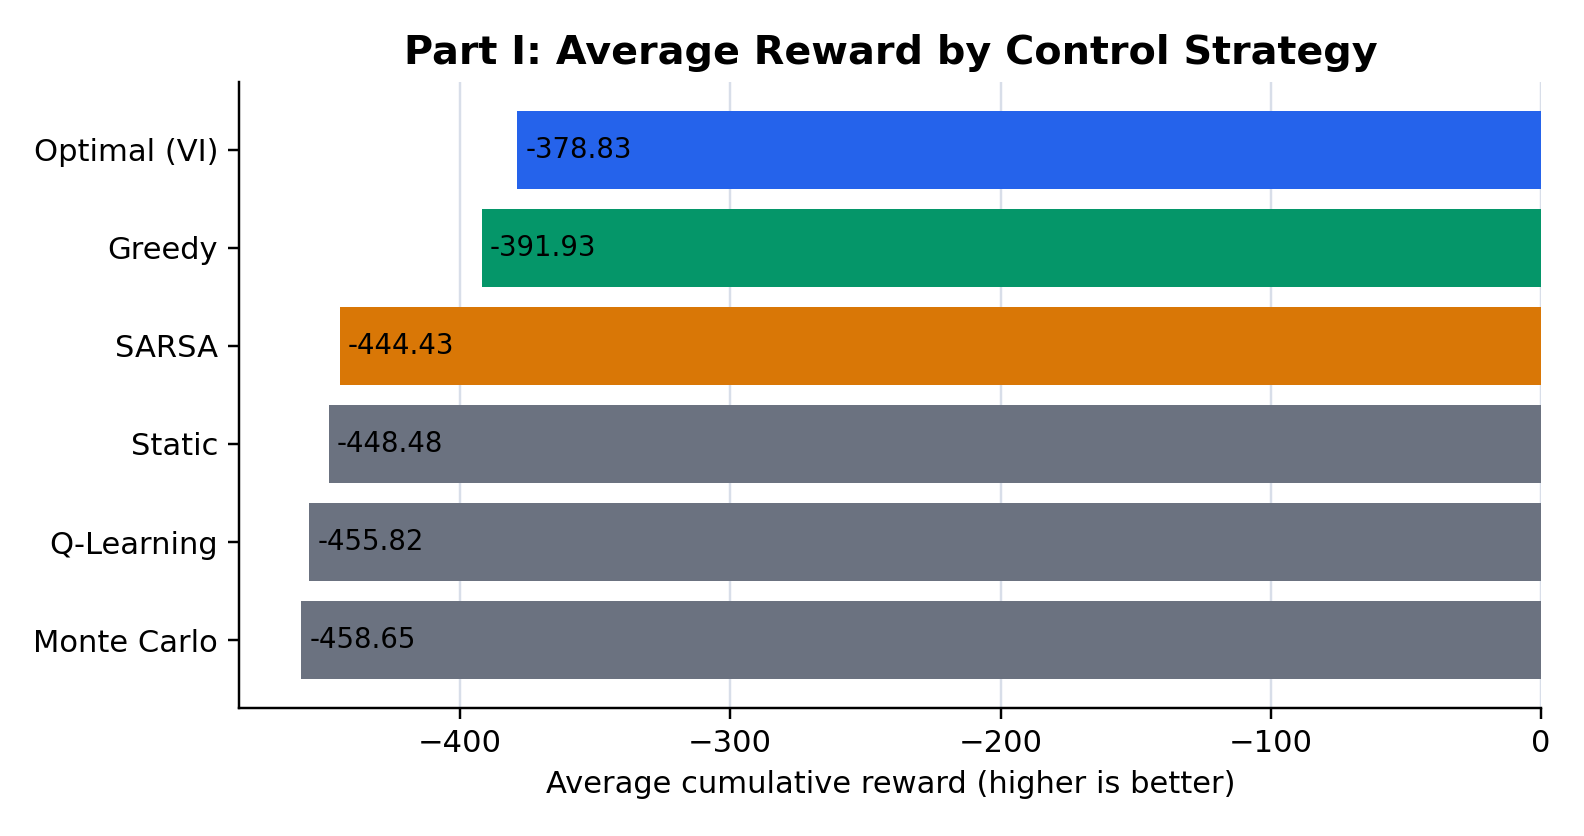
\includegraphics[width=0.62\linewidth]{figures/part1_reward_comparison.png}
\end{center}

\begin{center}
\begin{tabular}{lrr}
\toprule
Approach & Avg. Reward & Time \\
\midrule
Optimal (VI) & -378.83 & 0.24s \\
Greedy & -391.93 & 0.22s \\
SARSA & -444.43 & 0.85s \\
Static & -448.48 & 0.20s \\
Q-Learning & -455.82 & 1.16s \\
Monte Carlo & -458.65 & 5.81s \\
\bottomrule
\end{tabular}
\end{center}

In the simple single-intersection setting, SARSA slightly outperforms static timing, validating that reinforcement learning can learn useful adaptive policies. However, the greedy heuristic still performs strongly because the environment is simple and the heuristic has direct access to exact current queue information. This result does not refute RL; it shows that the benchmark is too local and too myopic to reveal RL's full advantage.

\section*{3. Extension: Coordinated Corridor}
To test richer traffic control, I added a two-intersection corridor. Vehicles released from Intersection A reach Intersection B after a four-step delay, demand changes by regime, and both lights must coordinate phases. The DQN observes queues at both intersections, phases, the in-transit vehicle bucket, and the demand regime. Static timing alternates on a fixed cycle. Greedy serves the larger current local queue and cannot anticipate platoons that are already in transit.

\begin{center}
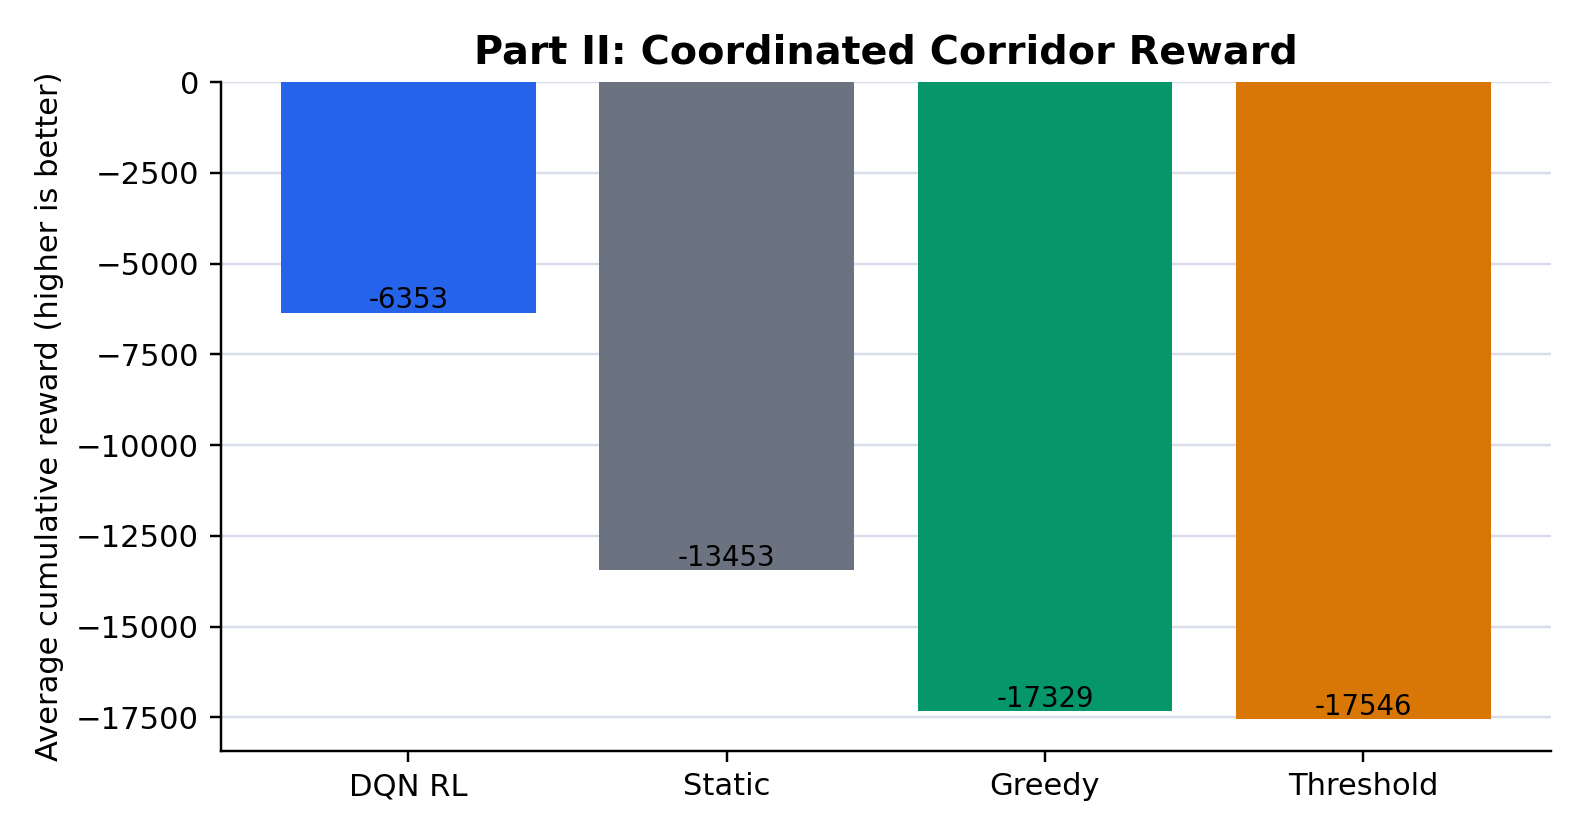
\includegraphics[width=0.54\linewidth]{figures/part2_reward_comparison.png}
\end{center}

\begin{center}
\begin{tabular}{lrrrr}
\toprule
Approach & Reward & Avg. Queue & Avg. Delay & Switches \\
\midrule
DQN RL & -6352.98 & 41.75 & 41.75 & 66.55 \\
Static & -13452.73 & 78.96 & 81.50 & 28.00 \\
Greedy & -17328.68 & 99.41 & 102.29 & 181.18 \\
Threshold & -17546.14 & 101.53 & 104.56 & 70.49 \\
\bottomrule
\end{tabular}
\end{center}

The extension shows that RL's advantage becomes clearer when the traffic system contains delayed interactions and coordination requirements that are difficult for reactive heuristics to capture. Greedy clears visible queues aggressively, but this causes downstream delay and frequent switching. DQN learns a more coordinated policy with lower queue-weighted delay. Future work should expand this toward continuous-state deep RL, multi-agent coordination, and larger road networks.

\clearpage
\bibliographystyle{plain}
\bibliography{references}

\clearpage
\appendix
\section*{Appendix: Reproducibility Notes}
The Part I figures are generated from the slide-exact CSV. The Part II DQN is trained with experience replay, a target network, epsilon-greedy exploration, and fixed evaluation seeds. Extra metrics and methodological details are stored in the \texttt{appendix/} directory.

\end{document}
